\documentclass[11pt]{article}
\usepackage{listings}
\usepackage[letterpaper]{geometry}
\usepackage{float}
\usepackage{graphicx}
\graphicspath{{./images/}}

\begin{document}

Morgan Rosenkranz 
EECE5644 
6/11/21 

\section*{Question 1:}

I started this question by defining the points of a cube and then assigning two of them as the means of each class.
I then gave each class two covariences which were just the identity matrix multiplied by a number between $0.4$ and $0.9$.

From there, I generated datasets of the different sample sizes given ($100,200,500,1000,2000,5000$), as well as a validation set of $100000$ samples.

I then used the means and covariences I created earlier to create an optimal classifier.
This optimal classifier uses the least expected risk with a 1-0 loss matrix to classify all the samples in the validation set.

Now that I had an classifier to compare with, I set about creating a classifier that uses multi-layer perceptrons.
I used k-fold cross validation to find the ideal number of perceptrons in the first hidden layer which were then passed to a softmax layer.
The figure below shows the variation in the number of perceptrons and the resulting probability of error using a model with that number of perceptrons on a dataset of the given size.

\begin{figure}[H]
	\centering
	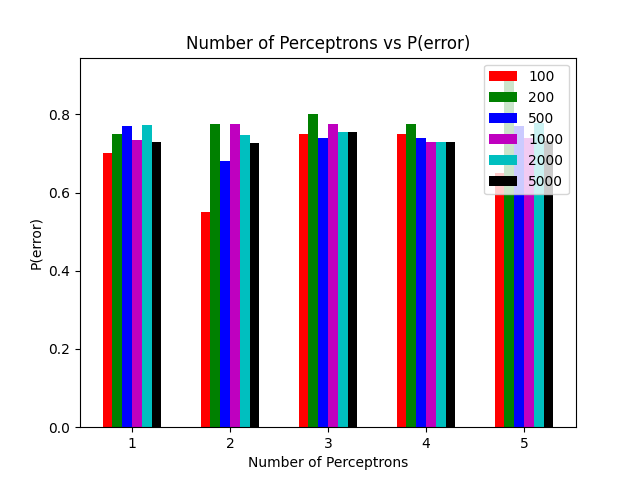
\includegraphics[width=0.75\textwidth]{perceptrons}
	\caption{Probability of Error Based on Sample Size and Number of Perceptrons Used}
\end{figure}

I then trained new models with the number of perceptrons that resulted in the least probability of error in for each sample set in the previous tests.
Finally, I used the validation set to test each model and compared the resulting probability of error with the optimal classifier:

\begin{figure}[H]
	\centering
	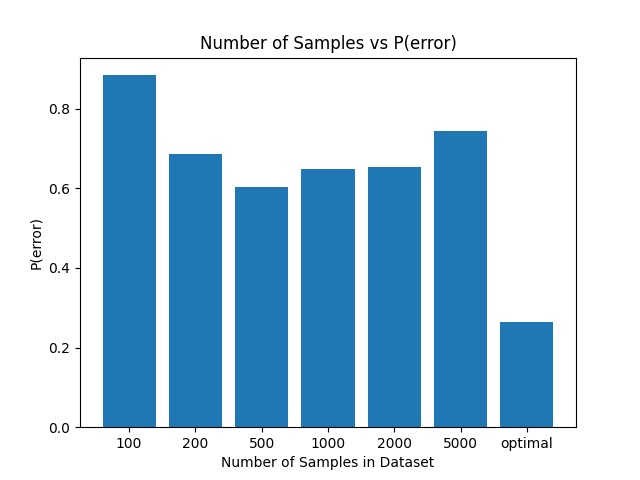
\includegraphics[width=0.75\textwidth]{samples}
	\caption{Performance of Models With Best Number of Perceptrons}
\end{figure}

No model performed nearly as well as the optimal classifier,
but it seems that the best performing case was a training set of 500 with 2 perceptrons.

\section*{Question 2:}
For this question I chose to use a Gaussian mixture of 6 randomly generated covariances, with evenly spaced means.
The covariances were created by multiplying the identity matrix with a random number between 0.1 and 0.5 to vary the size,
and then adding a slight variation in rotation by adding a random number between -1 and 1 to the other two values of the matrix.

I then created sample sets of $100, 1000, 10000, 100000$ and $1000000$.
I generated each set of samples for a given sample size 100 times so that I could use them later for multiple experiments without generating new samples.
Next I used both BIC and k-fold cross validation on each sample set with a gaussian model that was given an M value from 0 to 9.
I saved these sets to files for later analysis and the allow for parallel generation.
Even with a parallelized function, one million samples was just too many to train and validate with.
From the 100 experiments of each sample set I find which M had the best score for each trial and recorded it.
Using these M values I produced the following graphs:

\begin{figure}[H]
	\centering
	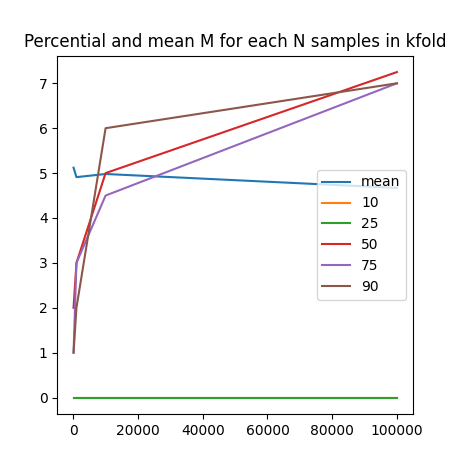
\includegraphics[width=0.75\textwidth]{kfoldper}
	\caption{}
\end{figure}

\begin{figure}[H]
	\centering
	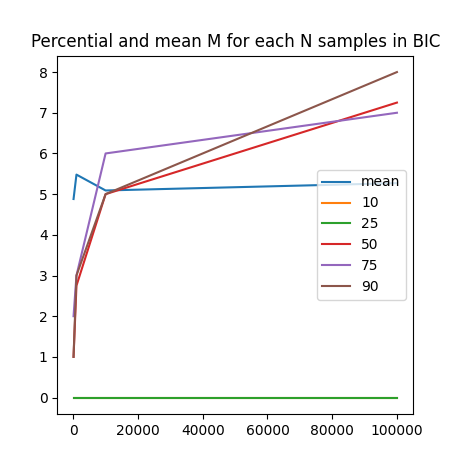
\includegraphics[width=0.75\textwidth]{bicper}
	\caption{}
\end{figure}

From these graphs we can see that by increasing the number of samples, the M values increased.
This makes sense but it doesn't seem to stablize around 6 as it should.

\section*{Code}
\subsection*{Code for Question 1}
\lstinputlisting[language=python]{q1.py}

\subsection*{Code for Question 2}
\lstinputlisting[language=python]{q2.py}
\end{document}
